\documentclass[12pt]{article}
\usepackage{setspace,graphicx,amsmath,geometry,fontspec,titlesec,soul,bm}
\titleformat{\section}[block]{\LARGE\bfseries}{\arabic{section}}{1em}{}[]
\titleformat{\subsection}[block]{\Large\bfseries\mdseries}{\arabic{section}.\arabic{subsection}}{1em}{}[]
\titleformat{\subsubsection}[block]{\normalsize\bfseries}{\arabic{subsection}-\alph{subsubsection}}{1em}{}[]
\titleformat{\paragraph}[block]{\small\bfseries}{[\arabic{paragraph}]}{1em}{}[]
\setmainfont{Times New Roman}
\renewcommand{\baselinestretch}{1.15}
\geometry{a4paper,left=2.5cm,right=2.5cm,top=2.5cm,bottom=2.5cm}
\begin{document}
	\newpagestyle{main}{            
		\sethead{Ziqing Yu}{Übugn 2}{3218051}     
		\setfoot{}{\thepage}{}     
		\headrule                                     
		\footrule                                       
	}
	\pagestyle{main}

\begin{figure}[ht]\centering
	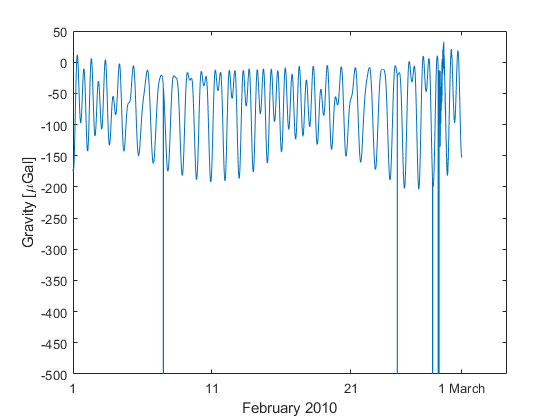
\includegraphics[width=1\textwidth]{grav.png}
	\caption{Periodogramm}
\end{figure}
\section{Was verursacht den Ausreißer in dieser Zeitreihe}
Die Messgeräte haben hohe Empfindlichkeit,daher übersteuert das Signal manchmal. D.h. das ist die technische Fehler in den Datensätze.
\section{Was sind die wichtigsten Gezeitenfrequenzen in dieser Zeitreihe}
Die wichtigsten Gezeitenfrequenzen in dieser Zietreihe sind halb Tag und 1 Tag wegen der Gravitation der Sonne und Mond
\section{Was verursacht die Hochfrequenzvariation in der Zeitreihe am 27. Februar}
Ein Erdbeben ist in dieser Zeitreihe passiert. (in Chile)
\section{Kann man durch die Analyse dieser Zeitreihe die hydrologischen Signale erkennen, Was sind die Frequenzen, die zuerst entfernt werden sollten}
Ja, man kann durch die Analyse dieser Zeitreihe die hydrologischen Signale erkennen. Die deutlich größere Periodedauern und kleinere Amplitude wie Gezeitenkräfte sollen zuerst entfernt werden.
\section{Dominanten Frequenzen}
\begin{figure}[ht]\centering
	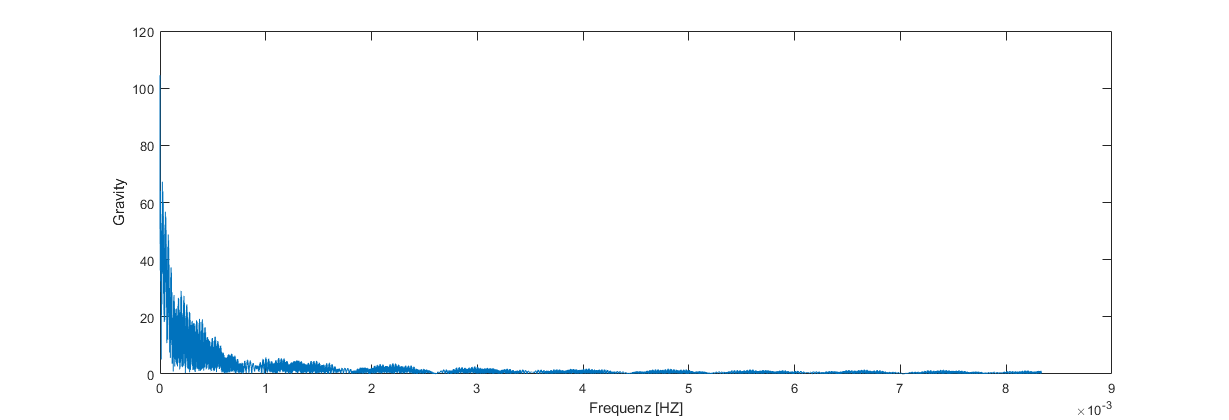
\includegraphics[width=1\textwidth]{fft.png}
	\caption{Periodogramm}
\end{figure}
Aus dem Graph ist es zu sehen, dass die Dominaten Frequenzen kleiner als $10^{-3} HZ$ sind, weil die Gezeitenfrequenzen kleiner als $10^{-3} HZ$ sind.
\end{document}